\documentclass[conference]{IEEEtran}
\IEEEoverridecommandlockouts
\usepackage{cite}
\usepackage{amsmath,amssymb,amsfonts}
\usepackage{algorithmic}
\usepackage{graphicx}
\usepackage{textcomp}
\usepackage{xcolor}
\usepackage{url}
\usepackage{booktabs}
\usepackage{multirow}
\usepackage{graphicx} % For resizebox

% Revision markup: changes made in response to the reviewers are shown in blue.
% For the clean camera-ready version, replace the definition below by \DeclareRobustCommand{\rev}[1]{#1}.
\DeclareRobustCommand{\rev}[1]{{\color{blue}#1}}

\def\BibTeX{{\rm B\kern-.05em{\sc i\kern-.025em b}\kern-.08em
    T\kern-.1667em\lower.7ex\hbox{E}\kern-.125emX}}

\begin{document}

\title{Adaptive Explanation Obfuscation via Reinforcement Learning}

\author{\IEEEauthorblockN{Gamze Erdoğan}
\IEEEauthorblockA{\textit{Istanbul Technical University}\\
Istanbul, Türkiye \\
gamze.erdogan@itu.edu.tr}
\and
\IEEEauthorblockN{Betül Güvenç-Paltun}
\IEEEauthorblockA{\textit{Ericsson}\\
Istanbul, Türkiye \\
betul.guvenc.paltun@ericsson.com}
\and
\IEEEauthorblockN{ Leyli Karaçay}
\IEEEauthorblockA{\textit{Ericsson}\\
Istanbul, T\"urkiye \\
leyli.karacay@ericsson.com}
\and
\IEEEauthorblockN{ Enver Ozdemir}
\IEEEauthorblockA{\textit{Istanbul Technical University}\\
Istanbul, Türkiye \\
ozdemiren@itu.edu.tr}
}

\maketitle

\begin{abstract}
Artificial intelligence (AI) models typically operate as opaque black boxes, producing outputs without revealing the reasoning behind them. This lack of transparency is undesirable, as clients submitting queries often require insight into how results are obtained. Explainable AI (XAI) addresses this need by providing interpretable explanations of model behavior. However, the very process of explanation can expose vulnerabilities: a malicious client may exploit explanations to extract sensitive information about the underlying model. Such model extraction attacks pose a significant threat to model owners, jeopardizing intellectual property and research investments. Consequently, developing robust defences against these attacks has become a critical area of research and in this work, we present solution to remedy such threats. The solution introduces a reinforcement learning (RL) agent that functions as a protective layer around an XAI model, dynamically adjusting the level of explanation provided based on ongoing interactions. The problem is structured as a continuous adversarial min-max game: an adversary attempts to reconstruct a surrogate model using the explanations given, while the RL agent actively obfuscates the explanations to prevent successful extraction. The system aims to satisfy legitimate user needs while penalizing the agent if the adversary successfully predicts or reconstructs the model. Over time, the agent learns to adapt its strategy, minimizing risks while maintaining the semantic usefulness of explanations for authorized users across varying model architectures.
\end{abstract}

\begin{IEEEkeywords}
Explainable AI (XAI), Reinforcement Learning (RL), Model Extraction Attacks, Privacy, Obfuscation.
\end{IEEEkeywords}

\section{Introduction}
Explainable Artificial Intelligence (XAI) focuses on making complex models and their predictions interpretable, providing insights into the reasoning processes behind machine learning outputs. However, while offering explanations assists legitimate users in comprehending model behavior, it simultaneously creates potential vulnerabilities that adversaries may leverage to replicate models.

A model extraction attack occurs when an adversary attempts to replicate a black box model. If an attack utilizes explanations, it is called an explanation-aware model extraction attack (XaMEA). In such attacks, the adversary sends a massive volume of crafted queries to reveal information about the target model's behavior. The explanations consist of additional information such as feature importance or confidence scores, which the attacker uses to match both the outputs and explanations of a surrogate model to those of the target model. Therefore,  when accompanied by explainability, even highly complex models remain vulnerable to extraction attacks.

To address these challenges, we introduce an approach that integrates a reinforcement learning (RL) agent with XAI to dynamically enhance privacy and security without strictly compromising the explanation quality for regular users.

\section{Related Work}
To contextualize our dynamic obfuscation approach, we review the literature across four key domains: model extraction vulnerabilities, the privacy-explainability trade-off, static defensive mechanisms, and the application of reinforcement learning in adversarial defense.

\subsection{Vulnerabilities in Machine Learning (Model Extraction)}
Standard machine learning models exposed via inference APIs are highly susceptible to model extraction (or model stealing) attacks \cite{b3, b5}. In these scenarios, adversaries systematically query the prediction API and utilize the resulting input-output pairs to train a functionally equivalent surrogate model \cite{b6}. Recent advances have demonstrated that these attacks can achieve both high accuracy and high fidelity representations of the target model \cite{b7}. This vulnerability extends beyond simple tabular classifiers, threatening complex sequential recommenders \cite{b2} and large language models \cite{b29}. Comprehensive surveys of the field emphasize that modern extraction methodologies are becoming increasingly query-efficient, drastically reducing the time and cost required for an adversary to steal proprietary intellectual property \cite{b30}.

\subsection{The Privacy-Explainability Trade-off and XaMEA}
The deployment of XAI methodologies, such as SHAP \cite{b12}, LIME \cite{b13}, and Integrated Gradients \cite{b14}, has become a standard practice for establishing algorithmic transparency. However, the literature increasingly recognizes a strict privacy-explainability trade-off \cite{b4}. Explanations inherently leak gradient information and expose local decision boundaries \cite{b16}. Milli et al. \cite{b8} theoretically and empirically demonstrated that gradient-based explanations allow for rapid, query-efficient model reconstruction.

This inherent vulnerability spawned the development of Explanation-Aware Model Extraction Attacks (XaMEA) \cite{b1}. By exploiting feature importances alongside standard outputs, attackers can accelerate the extraction process. Attack frameworks such as AUTOLYCUS \cite{b10} leverage model-agnostic tools like LIME and SHAP to infer decision boundaries with minimal queries, while similar architectures like Megrez \cite{b11} effectively target Deep Neural Networks. Furthermore, Shokri et al. \cite{b9} established that detailed explanations also exacerbate membership inference risks, confirming that transparency tools uniquely expose models to adversarial exploitation and manipulation \cite{b15}.

\subsection{Current Defensive Strategies and Their Limitations}
Mitigating model extraction traditionally relies on static defense mechanisms. Common techniques include Top-$k$ truncation \cite{b2}, which limits the informational bandwidth by restricting output dimensions, and prediction generalization, which obscures outputs through deliberate rounding \cite{b3}. More proactive defenses attempt to inject controlled, randomized noise into the API predictions \cite{b4, b20}, often drawing upon differential privacy (DP) frameworks \cite{b21} to provide mathematical privacy guarantees for interpretable models \cite{b22}.

Other state-of-the-art approaches, such as PRADA \cite{b17} and adaptive misinformation frameworks \cite{b18, b19}, analyze incoming query distributions to detect anomalous behavior and intentionally mislead attackers. However, when these static noise or truncation defenses are applied to XAI outputs, they inflict severe utility loss \cite{b4}. Static defenses cannot dynamically balance the conflicting needs of maintaining high explanation fidelity for benign users while securing the model against active adversaries.

\subsection{Reinforcement Learning in Adversarial Defense}
To effectively combat adaptive adversaries, defensive mechanisms must also be adaptive and unpredictable \cite{b28}. Reinforcement Learning (RL) has emerged as a powerful paradigm for addressing complex, dynamic challenges in cybersecurity \cite{b25}. Foundational algorithms like Deep Q-Networks (DQN) \cite{b24} and Proximal Policy Optimization (PPO) \cite{b23} have been successfully adapted for real-time threat detection and network intrusion mitigation \cite{b26}.

In the specific context of adversarial machine learning, frameworks like Robust Adversarial Reinforcement Learning (RARL) \cite{b27} formulate security as a continuous min-max game. This forces the RL agent to learn robust behavioral policies against active perturbations. By extending this game-theoretic RL approach to XAI obfuscation, our system overcomes the core limitations of static privacy mechanisms, allowing the model to dynamically optimize the trade-off between interpretability and security on a per-interaction basis.

\section{Proposed System Architecture}
The system consists of an inference provider who manages the ML model along with its associated explainability module. The RL agent acts as a protective mechanism that decides how much information to conceal or modify in an explanation.

\begin{figure}[htbp]
\centerline{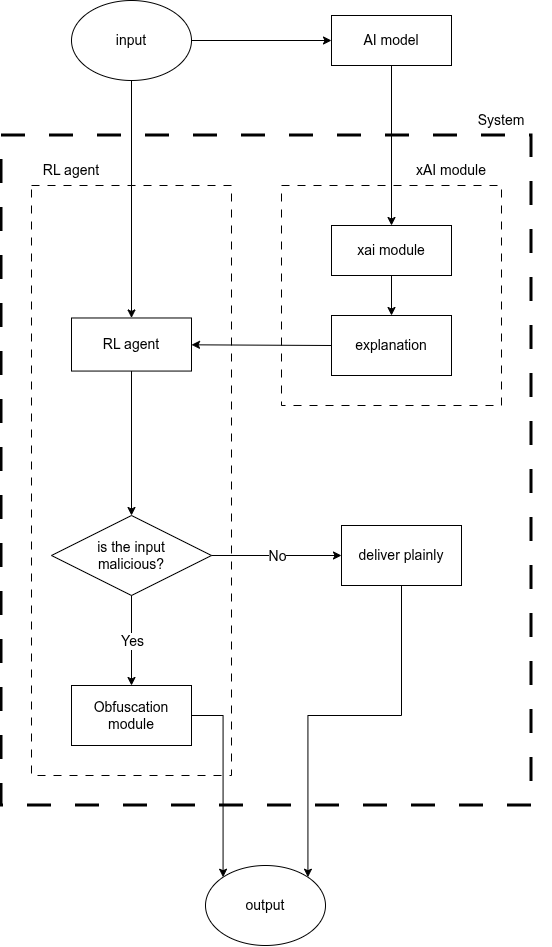
\includegraphics[width=\columnwidth]{fig1_overview.png}}
\caption{High-level overview of the system architecture.}
\label{fig1}
\end{figure}

As illustrated in Fig.~\ref{fig1}, the high-level components of the system are:
\begin{itemize}
    \item AI Model: A model hosted and served by the inference provider. In our evaluations, we utilize both Decision Tree Ensembles (XGBoost) and Deep Neural Networks (DNN) to demonstrate architectural generalizability.
    \item Input: The query submitted for processing.
    \item RL agent: Determines how much information to conceal in an explanation to limit model extraction while preserving utility. We utilize a Proximal Policy Optimization (PPO) algorithm for this agent.
    \item Obfuscation module: Intentionally obfuscates explanations to prevent attackers from learning too much about the model.
    \item XAI module: Generates baseline explanations for the outputs of the model using frameworks such as SHAP or LIME.
\end{itemize}

\begin{figure}[htbp]
\centerline{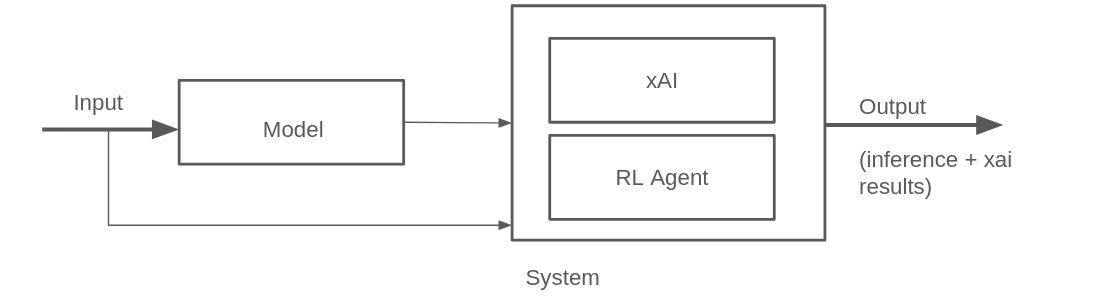
\includegraphics[width=\columnwidth]{fig2_workflow.png}}
\caption{System workflow: inference model output is explained by the XAI module and selectively obfuscated by the RL agent before returning results.}
\label{fig2}
\end{figure}

The workflow operates as follows (see Fig.~\ref{fig2}):
\begin{enumerate}
    \item An input query is submitted to the system.
    \item The input is processed on the model, generating an output.
    \item The input is simultaneously sent to the RL agent for analysis.
    \item The RL agent examines the input's relation to historical queries \rev{(through the rolling-window state of Eq.~(\ref{eq:state}))} and determines the degree of obfuscation required.
    \item The XAI module receives the output and generates a baseline explanation, which is sent to the RL agent.
    \item The RL agent decides whether to apply obfuscation to the explanation via the obfuscation module.
    \item The processed output and the (potentially obfuscated) explanation are returned to the user.
\end{enumerate}

\section{Game Design for the RL Agent}
\subsection{Reinforcement Learning Configuration}

\textbf{Algorithm Selection:}
To drive the dynamic obfuscation module, we employ the Proximal Policy Optimization (PPO) algorithm \cite{b23}. PPO was selected over alternative reinforcement learning algorithms, such as Deep Q-Networks (DQN) or Soft Actor-Critic (SAC), due to its inherent stability and compatibility with continuous action spaces. Because our obfuscation intensity $a_t$ is a continuous variable defined in the range $[0, 1]$, value-based methods like DQN, which require discrete action spaces, are unsuitable without arbitrary discretization. While SAC accommodates continuous actions, PPO's clipped surrogate objective function prevents destructively large policy updates, ensuring stable and monotonic improvement during the delicate min-max adversarial training process.

\textbf{State-Space Formulation and Network Architecture:}
The RL agent must make contextual decisions based on the current query and the history of adversarial interactions. \rev{The full history of a session (Eq.~(\ref{eq:history}) in Section~\ref{sec:game}) grows with every query, whereas an MLP policy requires an input of fixed size. We therefore encode the history in fixed size as a \emph{rolling window} of the user's last $k$ queries. Each query is first standardised with the training-set statistics, $z_t = (x_t - \bar{x})/\sigma_x$, and the state is the concatenation of the $k$ most recent standardised queries and the normalized step counter:}
\begin{equation}
\rev{s_t = \left[z_{t-k+1} \parallel \dots \parallel z_{t-1} \parallel z_t \parallel \frac{t}{T_{max}}\right]}
\label{eq:state}
\end{equation}
Where $t$ is the current query step and $T_{max}$ represents the maximum allowed queries in a session. \rev{At the start of a session ($t<k$), missing slots are filled with zeros (the feature mean). The size of $s_t$, $kd+1$ for $d$ features, is independent of $t$. The window preserves the order and recency of the user's queries, so the policy can condition on local query patterns such as bursts of near-duplicate or slightly perturbed queries, which session-wide averages would smooth out. We use $k=8$.} This combined vector is processed by the PPO agent, which is parameterized using a standard Multi-Layer Perceptron (MLP) architecture. The MLP network acts as both the actor, outputting the continuous action $a_t$, and the critic, estimating the state-value function to guide policy updates.

\textbf{Convergence Behavior:}
\rev{Each training episode is one simulated session of $T_{max}=1000$ queries, drawn in random order from a pool of 5,000 training samples; a new random session is drawn for every episode, so the agent cannot memorise a fixed query sequence.} Operating over 50,000 environmental timesteps \rev{(50 episodes)} with a learning rate of $3 \times 10^{-4}$, the agent \rev{learns a stable defensive policy}. Empirical learning curves derived from the environment's rolling episode rewards indicate that the agent steadily maximized its reward function, confirming that PPO effectively managed the volatile signals generated by the adversary's simultaneously evolving surrogate model. \rev{Performance is not yet saturated at this budget: training for 500,000 timesteps further improves the security of the learned policies (Section~\ref{sec:results}).}

The RL agent is trained using a game-based framework designed to enhance model security while maintaining explanation utility. The setup simulates a continuous adversarial scenario, as depicted in Fig.~\ref{fig3}.

\begin{figure}[htbp]
\centerline{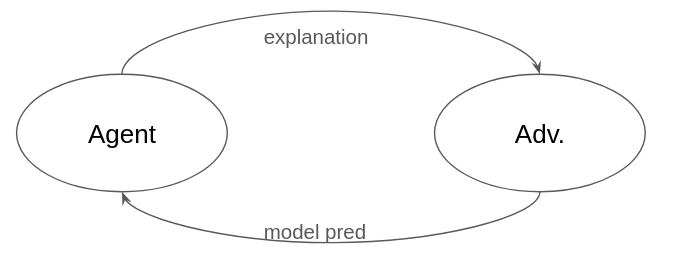
\includegraphics[width=\columnwidth]{fig3_training_loop.png}}
\caption{Game-based training loop: the RL agent obfuscates explanations; the adversary trains a surrogate model, and rewards/penalties are assigned based on security and explanation utility.}
\label{fig3}
\end{figure}

\subsection{Min-Max Game Formulation}
\label{sec:game}
\textbf{Step 1: State at time $t$}\\
The state $s_{i}$ at time $t$ is the history of queries received from a specific user, where $x_{i}$ is the query and $y_{i}$ is the output.
\begin{equation}
s_i = \{(x_1, y_1), (x_2, y_2), \dots, (x_i, y_i)\}
\label{eq:history}
\end{equation}
\rev{Eq.~(\ref{eq:history}) defines the information available to the defender; since it grows at every step, the agent observes it through the fixed-size encoding of Eq.~(\ref{eq:state}). The outputs $y_i = M(x_i)$ are a deterministic function of the queries and add no information, so the encoding keeps the queries only.}

\textbf{Step 2: RL Agent Action}\\
The RL agent determines an obfuscation function $f_{obfus}$ to apply to the true explanation $E_{true}$. The action $a_t$ is a continuous variable $a_t \in [0, 1]$ representing the intensity of obfuscation. The applied transformation is defined as:
\begin{equation}
E_{output} = (1 - a_t)E_{true} + a_t \cdot \epsilon
\end{equation}
Where $\epsilon$ represents Gaussian noise scaled by the standard deviation of the true explanations ($\epsilon \sim \mathcal{N}(0, \sigma_E^2)$). If $a_t = 0$, $E_{output} = E_{true}$ (full explanation). If $a_t = 1$, $E_{output}$ relies entirely on the generated noise (full obfuscation).

\textbf{Step 3: Adversary Action}\\
The adversary leverages $E_{output}$ to construct a surrogate model $S$ targeting the original model $M$. The adversary minimizes the extraction loss $L_{extract}$:
\begin{equation}
\min L_{extract}(S(x), M(x) | E_{output})
\end{equation}
\rev{The surrogate is trained incrementally: it is re-initialised at the start of every episode and updated with one gradient step per query on the input $[x_t, E_{output}]$ and label $M(x_t)$. $L_{extract}$ is the surrogate's cross-entropy with the target's labels on its $W=32$ most recent queries, measured before the update on $x_t$.}

\textbf{Step 4: Reward Function}\\
The reward function $R_t$ balances security (maximizing adversary loss) and utility (minimizing explanation deviation).
\begin{equation}
R_t = \lambda \cdot L_{extract}(S, M) - \mu \cdot \rev{\frac{||E_{true} - E_{output}||}{||E_{true}||}}
\end{equation}
Where $\lambda$ and $\mu$ are non-negative scalar hyperparameters weighing the importance of model security and explanation fidelity, respectively. \rev{The distortion term is normalized by $||E_{true}||$, as in the evaluation metric of Section~\ref{sec:metrics}, so that it is on the same scale as $L_{extract}$.}

\section{Experimental Evaluation}
\subsection{Experimental Setup}
To evaluate the proposed methodology and demonstrate its structural generalizability, we implemented two distinct machine learning pipelines:
\begin{enumerate}
    \item \textbf{Adult Income (XGBoost + SHAP):} A black-box XGBoost target model providing interpretability via SHAP TreeExplainer.
    \item \textbf{Credit Card Fraud (DNN + LIME):} A Deep Neural Network target model providing interpretability via LIME (Local Interpretable Model-agnostic Explanations).
\end{enumerate}

In both environments, the adversary was designed as an adaptive attacker aiming to replicate the target model using a surrogate Multi-Layer Perceptron (MLP) Classifier configured with two hidden layers of 64 and 32 neurons. The RL defending agent was trained independently for each pipeline using the PPO algorithm over 50,000 timesteps.

\rev{\textbf{Attackers.} The \emph{natural-query} attacker queries natural data in random order, as during training. The \emph{synthetic-query} attacker owns only 10 seed samples and generates new queries by perturbing earlier ones with random-sign steps of $0.1\sigma_x$ on a random subset of features, in the spirit of the augmentation-based attacks that PRADA \cite{b17} is designed to detect. All strategies are evaluated on the same three sessions of 500 held-out queries per attacker.}

\rev{\textbf{Agents.} Following the formulation of Section~\ref{sec:game}, we vary both weights: $\lambda \in \{0, 0.1, 0.25, 0.5, 0.75, 1, 1.5, 2, 3, 5\}$ at each $\mu \in \{0, 0.01, 0.05, 0.1, 0.2, 0.5\}$ (except $\lambda=\mu=0$). Each agent is trained with the rolling-window state of Eq.~(\ref{eq:state}) and, as an ablation, with the history-free state $s_t=[z_t \parallel t/T_{max}]$, over three random seeds; reported values are averages over the seeds.}

\subsection{Evaluation Metrics}
\label{sec:metrics}
We benchmark the defensive policies across three primary metrics to assess the balance between adversarial security and user interpretability:

\textbf{1. Average \rev{Adversary Error} ($L_{extract}$):} Measures the cross-entropy loss of the adversary's surrogate model. Higher values indicate successful defense against extraction. \rev{(We rename this metric from ``extraction loss'' because the defender maximizes it.)}

\textbf{2. Average \rev{Explanation Distortion} (L2 Distortion):} The normalized L2 norm between the true explanation and the obfuscated output, representing the raw geometric distortion.

\textbf{3. Semantic Interpretability Metrics:} To ensure the obfuscation policy does not destroy the inherent meaning of the explanations, we evaluate two semantic utility metrics:
\begin{itemize}
    \item \textit{Spearman's Rank Correlation ($\rho$):} Measures the monotonic relationship between the feature importance rankings of the original explanation $E_{true}$ and the obfuscated explanation $E_{output}$. A higher $\rho$ indicates that the relative hierarchy of feature importance is preserved.
    \item \textit{Top-$k$ Feature Agreement:} Calculates the intersection of the $k$ most critical features before and after obfuscation, defined as $\frac{|S_{true} \cap S_{output}|}{k}$, where $S$ represents the set of indices for the top $k$ features. We report results for $k=3$.
\end{itemize}

\subsection{Results and Baselines}
\label{sec:results}
The trained PPO agents were benchmarked against multiple static defense strategies prevalent in the literature: Top-$k$ truncation ($k=3$), Gaussian Noise addition (level=$0.5$), Precision Reduction ($2$ decimals), and Random Subset omission ($p=0.5$). \rev{We also compare against the state-of-the-art detector PRADA \cite{b17}, implemented from its published algorithm on standardised features. As PRADA detects rather than obfuscates, we use it as a gate: explanations are exact until the client is flagged and fully obfuscated ($a_t=1$) afterwards. Its threshold $\delta$ is the largest value that raises no alarm on benign sessions.}

\begin{table*}[t]
\caption{Security vs. Distortion Trade-off: Adult Income Dataset (XGBoost + SHAP)\rev{, natural-query attacker}}
\begin{center}
{\footnotesize
\begin{tabular}{lcccc}
\toprule
\textbf{Strategy} & \textbf{\rev{Adversary Error} $\uparrow$} & \textbf{\rev{Expl. Distortion} $\downarrow$} & \textbf{Spearman's $\rho$ $\uparrow$} & \textbf{Top-3 Agreement $\uparrow$} \\
\midrule
\multicolumn{5}{l}{\textit{Static Baselines}} \\
\rev{No Defense} & \rev{0.2345} & \rev{0.0000} & \rev{1.0000} & \rev{1.0000} \\
\rev{Precision Reduction (2 dec)} & \rev{0.2343} & \rev{0.0062} & \rev{0.9982} & \rev{0.9949} \\
\rev{Top-$k$ ($k=3$)} & \rev{0.2438} & \rev{0.1474} & \rev{0.9411} & \rev{1.0000} \\
\rev{Gaussian Noise (lvl=0.5)} & \rev{0.2521} & \rev{1.0688} & \rev{0.5901} & \rev{0.7211} \\
\rev{Random Subset (p=0.5)} & \rev{0.2758} & \rev{0.5883} & \rev{0.5575} & \rev{0.5471} \\
\rev{PRADA \cite{b17}} & \rev{0.2345} & \rev{0.0000} & \rev{1.0000} & \rev{1.0000} \\
\midrule
\multicolumn{5}{l}{\textit{RL Adaptive Agents ($\lambda=1.0$)\rev{, rolling-window state}}} \\
\rev{RL ($\mu = 0.1$)} & \rev{0.2536} & \rev{0.1607} & \rev{0.9128} & \rev{0.9447} \\
\rev{RL ($\mu = 0.05$)} & \rev{0.2651} & \rev{0.3763} & \rev{0.8140} & \rev{0.8977} \\
\rev{RL ($\mu = 0.01$)} & \rev{0.2795} & \rev{0.6804} & \rev{0.6876} & \rev{0.8396} \\
\rev{RL ($\mu = 0.0$)} & \rev{0.2826} & \rev{0.7535} & \rev{0.6588} & \rev{0.8264} \\
\midrule
\multicolumn{5}{l}{\rev{\textit{RL Adaptive Agents ($\lambda=1.0$), no history (ablation)}}} \\
\rev{RL ($\mu = 0.1$)} & \rev{0.2552} & \rev{0.0529} & \rev{0.9613} & \rev{0.9793} \\
\rev{\textbf{RL ($\mu = 0.05$)}} & \rev{\textbf{0.2717}} & \rev{\textbf{0.0813}} & \rev{\textbf{0.9351}} & \rev{\textbf{0.9704}} \\
\rev{RL ($\mu = 0.01$)} & \rev{0.2912} & \rev{0.4182} & \rev{0.7567} & \rev{0.8613} \\
\rev{RL ($\mu = 0.0$)} & \rev{0.3007} & \rev{0.9864} & \rev{0.5178} & \rev{0.7407} \\
\bottomrule
\end{tabular}
}
\label{tab_adult}
\end{center}
\end{table*}

\begin{table*}[t]
\caption{Security vs. Distortion Trade-off: Credit Card Fraud Dataset (DNN + LIME)\rev{, natural-query attacker}}
\begin{center}
{\footnotesize
\begin{tabular}{lcccc}
\toprule
\textbf{Strategy} & \textbf{\rev{Adversary Error} $\uparrow$} & \textbf{\rev{Expl. Distortion} $\downarrow$} & \textbf{Spearman's $\rho$ $\uparrow$} & \textbf{Top-3 Agreement $\uparrow$} \\
\midrule
\multicolumn{5}{l}{\textit{Static Baselines}} \\
\rev{No Defense} & \rev{0.0866} & \rev{0.0000} & \rev{1.0000} & \rev{1.0000} \\
\rev{Precision Reduction (2 dec)} & \rev{0.0851} & \rev{0.5643} & \rev{0.7728} & \rev{0.4438} \\
\rev{Top-$k$ ($k=3$)} & \rev{0.0822} & \rev{0.7632} & \rev{0.5287} & \rev{1.0000} \\
\rev{Gaussian Noise (lvl=0.5)} & \rev{0.0812} & \rev{0.7064} & \rev{0.7967} & \rev{0.5256} \\
\rev{Random Subset (p=0.5)} & \rev{0.0933} & \rev{0.6977} & \rev{0.6469} & \rev{0.4987} \\
\rev{PRADA \cite{b17}} & \rev{0.0866} & \rev{0.0000} & \rev{1.0000} & \rev{1.0000} \\
\midrule
\multicolumn{5}{l}{\textit{RL Adaptive Agents ($\lambda=1.0$)\rev{, rolling-window state}}} \\
\rev{RL ($\mu = 0.1$)} & \rev{0.0863} & \rev{0.3000} & \rev{0.8524} & \rev{0.8082} \\
\rev{RL ($\mu = 0.05$)} & \rev{0.0859} & \rev{0.4240} & \rev{0.7856} & \rev{0.7401} \\
\rev{RL ($\mu = 0.01$)} & \rev{0.0848} & \rev{0.5319} & \rev{0.7295} & \rev{0.6859} \\
\rev{RL ($\mu = 0.0$)} & \rev{0.0847} & \rev{0.5440} & \rev{0.7231} & \rev{0.6788} \\
\midrule
\multicolumn{5}{l}{\rev{\textit{RL Adaptive Agents ($\lambda=1.0$), no history (ablation)}}} \\
\rev{RL ($\mu = 0.1$)} & \rev{0.0864} & \rev{0.0250} & \rev{0.9913} & \rev{0.9840} \\
\rev{RL ($\mu = 0.05$)} & \rev{0.0864} & \rev{0.0674} & \rev{0.9739} & \rev{0.9550} \\
\rev{RL ($\mu = 0.01$)} & \rev{0.0869} & \rev{0.2622} & \rev{0.8806} & \rev{0.8186} \\
\rev{RL ($\mu = 0.0$)} & \rev{0.0870} & \rev{0.3842} & \rev{0.8186} & \rev{0.7484} \\
\bottomrule
\end{tabular}
}
\label{tab_credit}
\end{center}
\end{table*}

\rev{\textit{Correction.} In the original submission, the adversary error was set to a constant 1.0 whenever the adversary's 32-query window contained a single class, which is almost always the case on the highly imbalanced Credit Card Fraud data; this produced its uniform values of 0.98--0.99. All results in this version are recomputed with the corrected metric.}

As demonstrated in Table \ref{tab_adult}, static methods struggle to balance the tradeoff effectively on the SHAP pipeline. While Gaussian Noise and Random Subset methods exhibit higher security, they inflict severe utility loss (\rev{1.0688 and 0.5883}, respectively), rendering the explanations functionally useless for benign users. In contrast, the RL Agent ($\mu=0.05$) successfully increases security (\rev{0.2717}) over the baseline (\rev{0.2345}, \rev{+16\%}) while maintaining an exceptional explanation fidelity (Top-3 Agreement $\approx 0.97$). \rev{It thus nearly matches the security of Random Subset (0.2758) at one seventh of its distortion, and is more secure than Gaussian Noise at less than a tenth of its distortion. Fig.~\ref{fig_pareto} shows the complete trade-off for both datasets.}

\rev{\textbf{Varying $\lambda$.} Fig.~\ref{fig_lambda} reports all four metrics as a function of the security weight $\lambda$. On Adult Income, increasing $\lambda$ raises the adversary error from the undefended 0.2345 to about 0.28 while distortion grows and the rank metrics decrease, i.e.\ $\lambda$ moves the agent along the security--utility trade-off. Since multiplying $R_t$ by a positive constant does not change the optimal policy, the trade-off depends on the ratio $\lambda/\mu$, which our grid confirms: for example, the no-history agents with $(\lambda,\mu) = (0.25, 0.01)$, $(1, 0.05)$ and $(2, 0.1)$, all with $\lambda/\mu=20$, reach adversary errors of 0.274, 0.272 and 0.270 at distortions of 0.09, 0.08 and 0.09.}

\rev{\textbf{Comparison with PRADA.} PRADA never flags the natural-query attacker, whose queries are, by construction, indistinguishable from those of a benign client (Tables~\ref{tab_adult} and~\ref{tab_credit}). Against the synthetic-query attacker it is effective but coarse (Table~\ref{tab_synth}): it flags the client at query 101--102, the earliest point its statistical test allows, and fully obfuscates everything afterwards. On Adult Income, the RL agent ($\lambda=1$, $\mu=0.01$, no history) comes close to PRADA's security (0.1898 vs.\ 0.2101) at one sixth of its distortion (0.24 vs.\ 1.49), while preserving the feature ranking ($\rho=0.85$ vs.\ 0.20). The two defenses are complementary. Unlike detection-based defenses such as PRADA, which cannot identify attackers that query natural data, the RL agent protects against both attacker types. Against synthetic-query attackers, PRADA attains the highest security but destroys the explanations once triggered, whereas the RL agent attains comparable security at a fraction of the distortion. PRADA, in turn, releases exact explanations to clients it does not flag, whereas the RL agent studied here obfuscates for every client (see below).}

\begin{table}[t]
\caption{\rev{Synthetic-Query Attacker: Adversary Error ($\uparrow$) / Explanation Distortion ($\downarrow$)}}
\begin{center}
\rev{
\begin{tabular}{lcc}
\toprule
\textbf{Strategy} & \textbf{Adult Income} & \textbf{Credit Card} \\
\midrule
No Defense & 0.1259 / 0.00 & 0.0627 / 0.00 \\
Random Subset (p=0.5) & 0.1808 / 0.59 & 0.0685 / 0.70 \\
PRADA \cite{b17} & 0.2101 / 1.49 & 0.0623 / 1.44 \\
\midrule
\multicolumn{3}{l}{\textit{RL ($\lambda=1$), rolling-window state}} \\
RL ($\mu = 0.05$) & 0.1530 / 0.24 & 0.0633 / 0.30 \\
RL ($\mu = 0.01$) & 0.1742 / 0.55 & 0.0638 / 0.38 \\
\multicolumn{3}{l}{\textit{RL ($\lambda=1$), no history (ablation)}} \\
RL ($\mu = 0.05$) & 0.1567 / 0.08 & 0.0629 / 0.12 \\
RL ($\mu = 0.01$) & 0.1898 / 0.24 & 0.0634 / 0.37 \\
\bottomrule
\end{tabular}
}
\label{tab_synth}
\end{center}
\end{table}

\rev{\textbf{Effect of the query history.} Across both datasets and attackers, the rolling-window agent does not reach a better trade-off than the history-free ablation: at equal distortion, the no-history agent is at least as secure (Fig.~\ref{fig_pareto}). This is expected in the game studied here: every training session is an extraction attempt with independently drawn queries, so earlier queries carry no information about the current one, while the larger input makes the policy harder to learn. This is not an artefact of the training budget: at 500,000 timesteps ($\lambda=1$, $\mu=0.05$), the no-history agent reaches an adversary error of 0.3015 (+29\% over no defense) at a distortion of 0.14 ($\rho=0.88$, Top-3 agreement 0.95) on Adult Income, and 0.1991 at a distortion of 0.19 against the synthetic-query attacker, whereas the rolling-window agent reaches 0.2671 at a distortion of 0.33. The history encoding becomes relevant when benign and malicious clients are served by the same agent, so that past queries indicate which kind of client is being served; we leave this setting to future work. Relatedly, as the agent is trained only on extraction sessions, it applies the same obfuscation to benign clients, who therefore bear the distortion reported above; training on mixed sessions, rewarding exact explanations for benign clients, is the natural remedy.}

The evaluation on the Credit Card Fraud dataset (Table \ref{tab_credit}) further demonstrates the severe limitations of static defenses when applied to LIME explanations. While Top-$k$ Truncation ($k=3$) maintains perfect Top-3 Agreement, it completely disrupts the overall feature ranking ($\rho \approx \rev{0.53}$). Conversely, Precision Reduction preserves general ranking ($\rho \approx \rev{0.77}$) but loses over half of the most critical top-3 features (Agreement $\approx \rev{0.44}$). \rev{Our adaptive policy ($\lambda=1.0, \mu=0.05$, no history) maintains high rank correlation ($\rho \approx 0.97$) and preserves the most critical features (Top-3 Agreement $\approx 0.96$). However, on this dataset no defense, static or adaptive, yields a meaningful security gain: the adversary error stays between 0.081 and 0.093 for every strategy. Fraud accounts for only 0.17\% of the transactions, so sessions of natural queries contain almost no positive cases and a surrogate that predicts the majority class imitates the target well regardless of the explanations. The RL agents learn that obfuscation does not pay here and keep the distortion low. Defending explanations of models trained on highly imbalanced data therefore requires a threat model with class-balanced queries, which we leave to future work.}

\begin{figure*}[t]
    \centering
    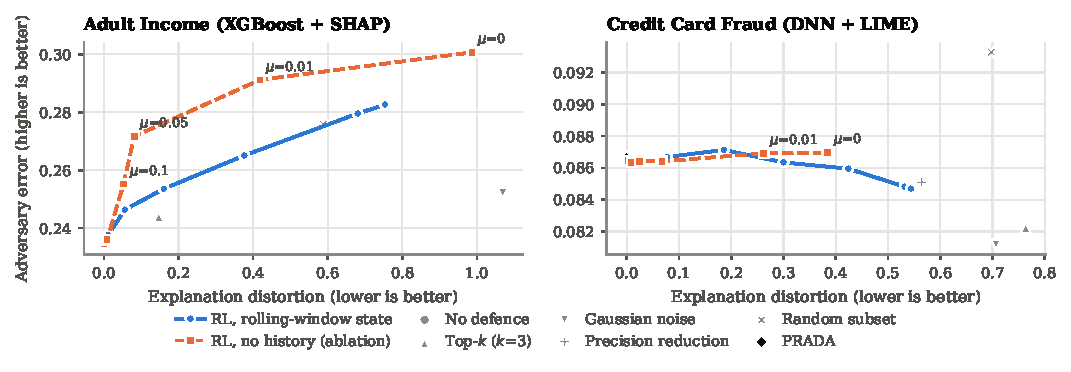
\includegraphics[width=\textwidth]{fig4_tradeoff.pdf}
    \caption{Security versus Distortion \rev{trade-off for both datasets (natural-query attacker). RL agents use $\lambda=1$ with $\mu$ varied, averaged over three seeds; static baselines and PRADA are shown for reference.}}
    \label{fig_pareto}
\end{figure*}

\begin{figure*}[t]
    \centering
    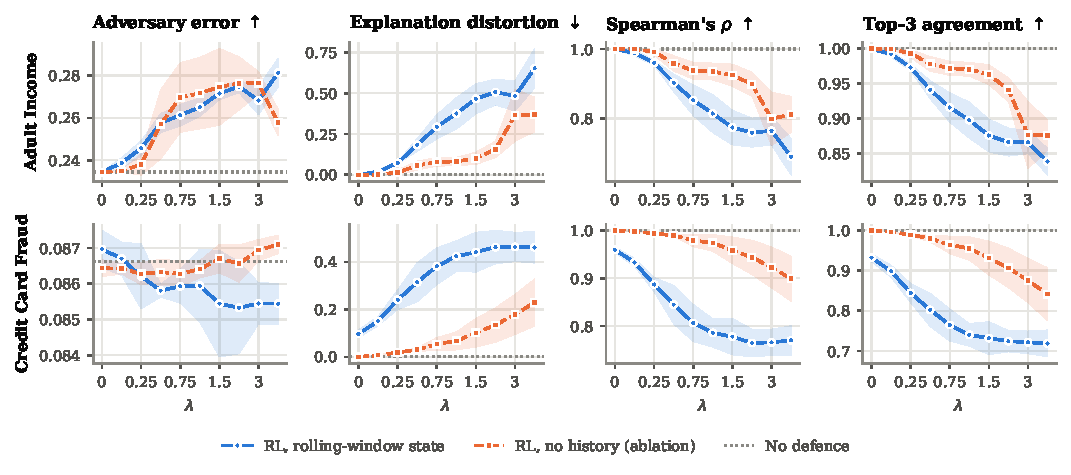
\includegraphics[width=\textwidth]{fig5_lambda_sweep.pdf}
    \caption{\rev{All four metrics as a function of the security weight $\lambda$ ($\mu=0.05$, natural-query attacker), for the rolling-window state and the no-history ablation; mean $\pm$ standard deviation over three seeds. Note the narrow adversary-error range on Credit Card Fraud.}}
    \label{fig_lambda}
\end{figure*}

\section{Discussion and Practical Deployment}

\subsection{Addressing Computational Overhead}
A primary concern when integrating adaptive defense mechanisms into production machine learning pipelines is the introduction of unacceptable latency during real-time inference. Traditional reinforcement learning training is computationally intensive; however, the deployment phase of our proposed architecture introduces \rev{little} overhead.

The trained PPO actor is parameterized as a lightweight Multi-Layer Perceptron (MLP). During inference, calculating the obfuscation intensity $a_t$ requires only a single forward pass through this shallow neural network. \rev{We measured the per-query cost on a single CPU core (median over all evaluation queries; Table~\ref{tab_timing}). The RL defense (state encoding, policy forward pass and obfuscation) takes 0.34~ms, less than PRADA. It adds only 2.3\% to LIME explanations; with the much faster TreeSHAP it adds 56\%, yet a query is still served in about 1.2~ms.} Therefore, the dynamic obfuscation layer can be deployed as an API gateway proxy without violating strict latency service-level agreements (SLAs).

\begin{table}[t]
\caption{\rev{Time per Query (ms, median, single CPU core); in parentheses, the defense's cost relative to explanation generation}}
\begin{center}
\rev{
\footnotesize
\begin{tabular}{lcc}
\toprule
\textbf{Component} & \textbf{Adult (SHAP)} & \textbf{Credit (LIME)} \\
\midrule
\multicolumn{3}{l}{\textit{Serving the query}} \\
Model prediction & 0.30 & 0.20 \\
Explanation & 0.61 & 15.09 \\
\midrule
\multicolumn{3}{l}{\textit{Defense}} \\
No Defense & 0.002 (0.4\%) & 0.002 (0.0\%) \\
Precision Reduction (2 dec) & 0.008 (1.4\%) & 0.009 (0.1\%) \\
Random Subset (p=0.5) & 0.010 (1.7\%) & 0.010 (0.1\%) \\
Top-$k$ ($k=3$) & 0.010 (1.7\%) & 0.011 (0.1\%) \\
Gaussian Noise (lvl=0.5) & 0.022 (3.7\%) & 0.023 (0.2\%) \\
PRADA \cite{b17} & 0.44 (73\%) & 0.46 (3.1\%) \\
RL, no history & 0.34 (56\%) & 0.34 (2.3\%) \\
RL, rolling-window state & 0.34 (56\%) & 0.35 (2.3\%) \\
\bottomrule
\end{tabular}
}
\label{tab_timing}
\end{center}
\end{table}

\subsection{Dynamic Threat Posturing}
The ablation study demonstrates that a single RL architecture can accommodate diverse security postures. In a practical deployment, a centralized security orchestration system could dynamically swap the active RL agent weights based on the current global threat level. During periods of normal operation, the system can utilize a high-utility agent ($\mu = 0.05$). If an intrusion detection system (IDS) flags an ongoing distributed XaMEA attack, the gateway can instantly pivot to a high-security agent ($\mu = 0.01$), actively stifling the extraction attempt while still providing baseline, albeit noisy, interpretability.

\section{Advantages of the Proposed Solution}
The dynamic integration of the RL agent provides several technical benefits:
\begin{itemize}
    \item \textbf{Enhanced Security:} Mitigates model extraction attacks by limiting explanation detail during suspicious activity.
    \item \textbf{Adaptive Explanations:} Continuously monitors query patterns and adapts the detail level based on historical interactions.
    \item \textbf{Balanced Utility:} As evidenced by the empirical benchmarks, authorized users receive high-quality insights with negligible semantic distortion, while adversaries are successfully stifled.
    \item \textbf{Robustness:} The RL agent adapts over time \rev{and applies unchanged} across varied architectures (Tree Ensembles and DNNs) and XAI methods (SHAP and LIME)\rev{; where obfuscation cannot improve security, as on the highly imbalanced Credit Card Fraud data, it learns to preserve explanation utility instead}.
\end{itemize}

\section*{Acknowledgment}
The authors acknowledge the use of generative AI tools (specifically, large language models) to assist with code optimization, script debugging, and language proofreading during the preparation of this manuscript. All AI-assisted outputs were thoroughly reviewed, edited, and validated by the human authors, who take full and final responsibility for the originality, accuracy, and integrity of this work.

\bibliographystyle{IEEEtran}
\bibliography{references}


%\begin{thebibliography}{00}

%\end{thebibliography}
\end{document}
